\begin{frame}[t]{¿Y después?}
\begin{itemize}
  \item Ya estamos trabajando en C++20:
    \begin{itemize}
      \item Mejor programación genérica con \textgood{conceptos} {B. Stroustrup et al.}
      \item Mejor procesamiento asíncrono con \textgood{corrutinas} {G. Nishanov}
      \item Mejor estructuración con \textgood{módulos} {G. Dos Reis}
      \item Mejor detección de defectos con \textgood{contratos} {J. Daniel García}
      \item \ldots
    \end{itemize}
\end{itemize}
\end{frame}

\begin{frame}[t]{Resumen}
\begin{itemize}[<+->]
  \item Limpieza de características antiguas.
  \item C++ es un lenguaje en constante evolución.
  \item Un lenguaje algo más predecible.
  \item Mejor soporte (ligeramente) de programación genérica.
  \item Mayor uso de atributos.
  \item Simplificaciones en el lenguaje para código más claro.
  \item Algoritmos paralelos y acceso al sistema de fichero.
  \item Algunos tipos nuevos en la biblioteca.
\end{itemize}
\end{frame}

\begin{frame}[t]{Si quieres más C++}
\begin{itemize}
  \item \cppid{\url{https://usingstdcpp.org/}}
\end{itemize}
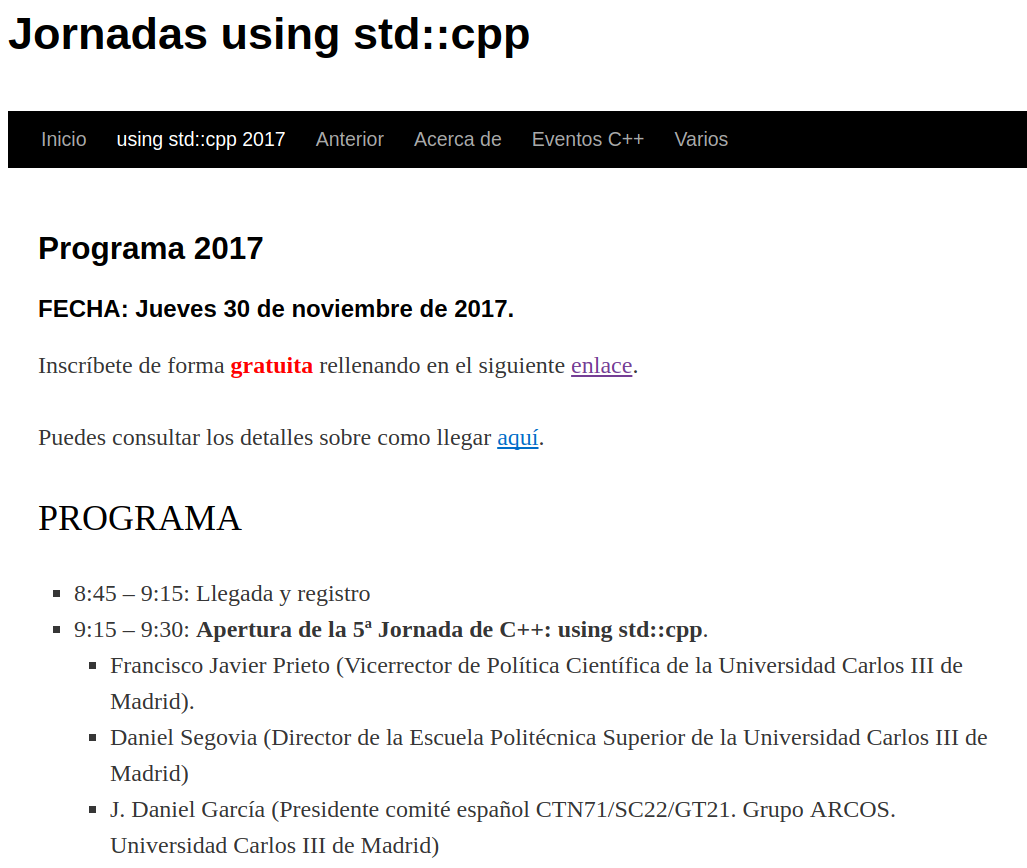
\includegraphics[width=\textwidth]{../img/using.png}
\end{frame}

\begin{frame}[t]{La fundación C++}
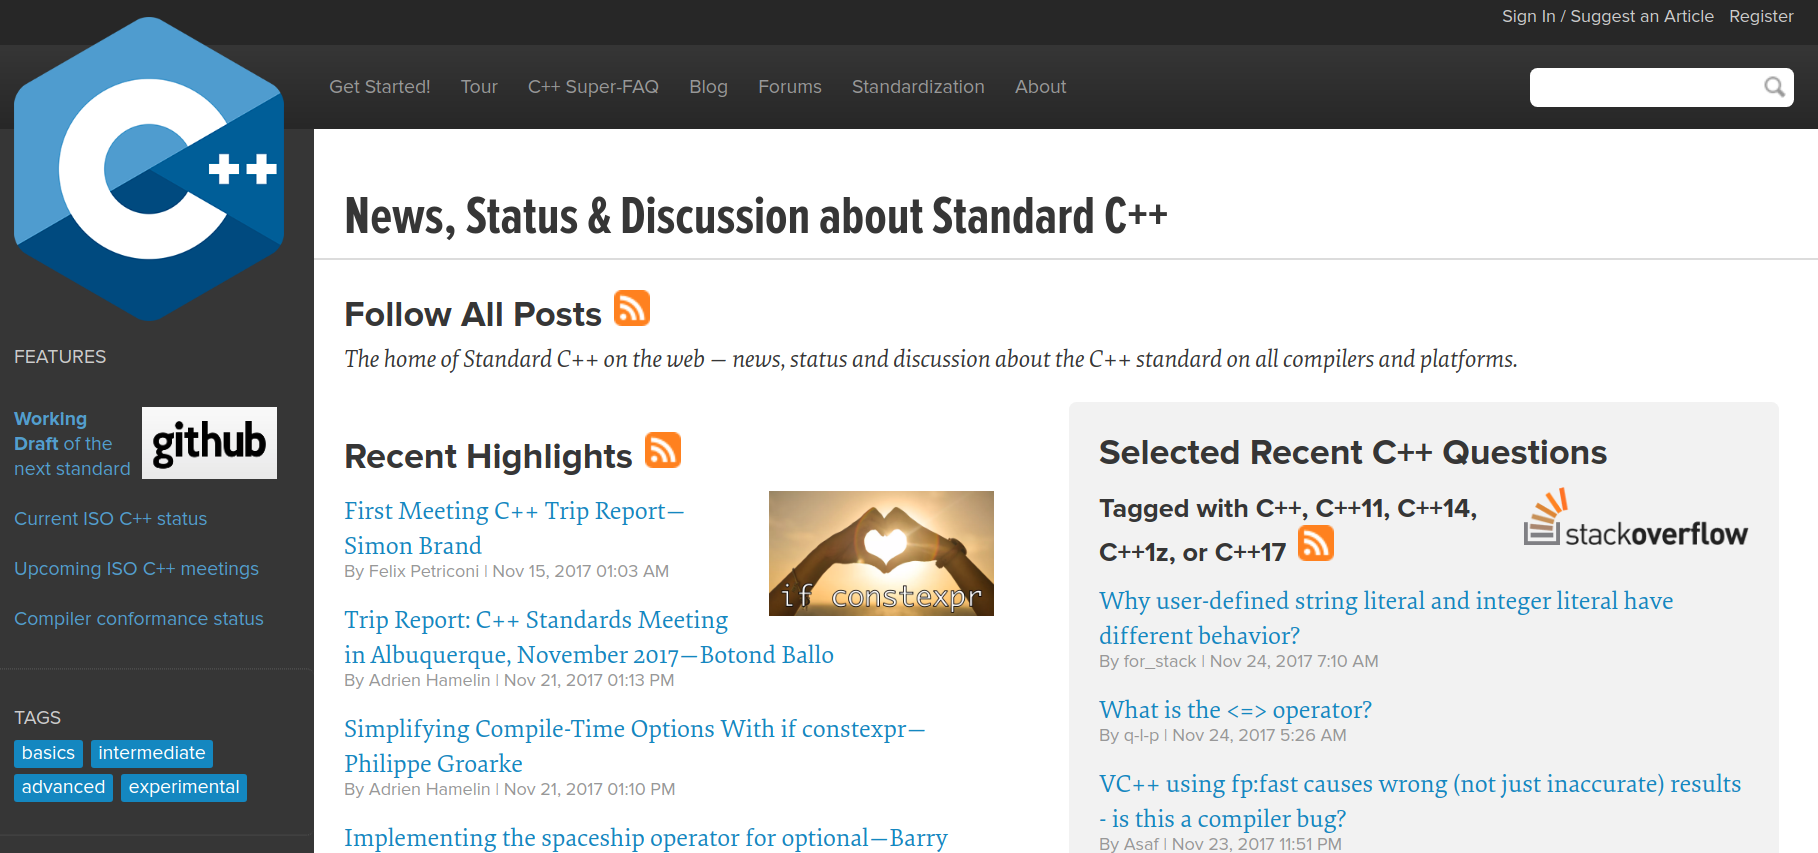
\includegraphics[width=\textwidth]{../img/isocpp.png}
\end{frame}

\begin{frame}[t]{No olvidéis}
\vfill
\begin{Huge}
\begin{center}
\textgood{¡¡¡Dadme feedback!!!}
\end{center}
\end{Huge}
\vfill
\end{frame}
